\documentclass[pdftex]{article}
% \documentclass[prl,showpacs,amsmath,amssymb]{revtex4} % PRL

% margins of 1 inch:
\setlength{\topmargin}{-.5in}
\setlength{\textheight}{9in}
\setlength{\oddsidemargin}{0in}
\setlength{\textwidth}{6.5in}

\usepackage[pdftex]{hyperref} % hyperlink equation and bibliographic citations
\usepackage[dvips]{graphicx,color}
\usepackage{amsmath} % advanced math
\usepackage{verbatim} % multi-line comments
\usepackage[numbers]{natbib} % bibilography
\usepackage{mciteplus} % collapse multiple citations in bibilography

% from http://www.flakery.org/search/show/569

\newcommand{\infint}{\ensuremath{\int_{-\infty}^{\infty}}}

\newcommand{\ie}{\textit{i.e.}\ }
\newcommand{\eg}{\textit{e.g.}\ }

\newcommand{\eqn}[1]{Eq.\ (\ref{#1})}

\newcommand{\pfrac}[2]{\ensuremath{\frac{\partial #1}{\partial #2}}}

\begin{document}

\title{Network Topology Optimization}

\author{Ben Payne$^{1}$\footnote{Electronic address: bpayne@lps.umd.edu}
{\it $^{1}$Department of Fun, University Name \& Town, city, State Zip}}

\date{\today}

\begin{abstract}
Three important factors when designing a network topology for a High Performance Computer system are time-to-solution, cost, and resiliance. The number of possible designs is very large for clusters of Exascale size. Here the time-to-solution is with respect to a specific application requirement, simultaneous all-to-all communication and small messages. Average time-to-solution is compared to modified graph-centric metrics average hop count and the bisection count.
\end{abstract}

%\maketitle % declares end of title page

\tableofcontents

%\newpage

\section{Introduction}

What is the best network topology for simultaneous all-to-all communication?

Currently implemented topologies, i.e., Butterfly, Dragonfly, are better for certain applications compared to other options, i.e., Mesh or Toroidal. However, showing a given network design to be analytically optimal for any one task, much less a combination of objectives, is difficult. In this study, a method for searching for an optimal topology with respect to multiple goals is described. An evolutionary search technique, simulated annealing, is proposed to determine network designs which are tailored to the needs of a specific application and set of user-defined goals. These objectives can include cost, time-to-solution, and reliability.

\section{Method}

In order to find network topologies specifically designed for narrow use cases, two approaches are taken. In the first, compute nodes are distingished from router nodes on an undirected graph. Rather than considering network traffic and router algorithms, only graph-based metrics are used: the hop count distribution and minimum bisection count. Each of these two must be defined in the context of a graph with two distinct types of nodes -- compute nodes from which information is sent and received, and router nodes which only redirect information. 
% From this study we show that random graphs, uniform lattices, and scale-free graphs converge to ?

In the second approach, a more realistic method is used. 
%Rather than randomly generating the network of compute and router nodes, it is assumed that compute nodes and first router share a common design. This assumption is based on normal manufacturing procedures of producing homogeneous components. 
Since the time-to-solution is the most direct measure of quality for a network topology, a more detailed simulation is needed. The need for timing requires that traffic congestion be included, which necessitates routing algorithms be specified. A cycle-accurate network simulator, SST/macro, is used to carry out the bucket sort algorithm. 

% describe simulated annealing technique
% discuss valid mutations; preserve symmetry or introduce randomness? Valid network 
% what other options are their for the evolutionary search?
% why not brute force search?
% why not analytical search?
\begin{figure}
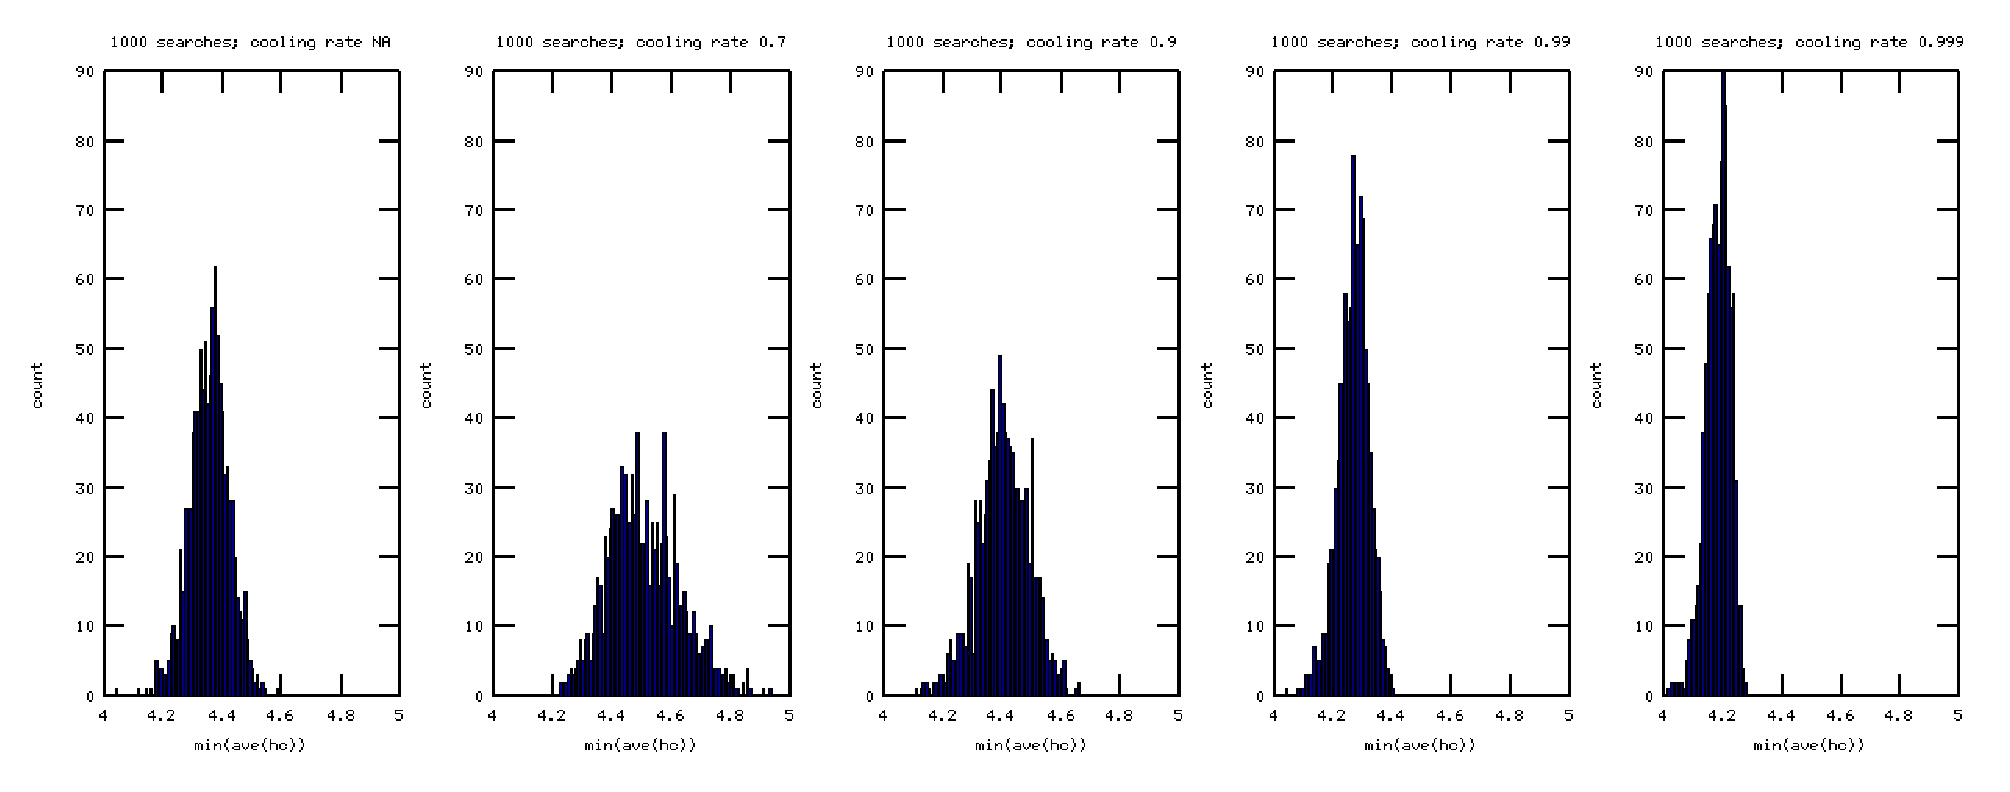
\includegraphics[scale=0.5]{pictures/Simulated_annealiing_OFF_and_ON_comparison_of_cooling_rates_1000searches}
\caption{Simulated annealing off (left-most histogram) and on for various cooling rates. Higher cooling rate results in slower annealing process. Each histogram is 1000 searches, starting from a 4x4 mesh grid and reducing the average hop count between compute nodes..}
\end{figure}


\section{Questions}

\textit{Choice of fitness function: Does the minimum bisection count and average hop count yield the same solution as the average time-to-solution?}

To measure this, we set up a highly asymmetric network composed of two connected routers. One router is connected to one computer, and the other router is connected to 7 other computers. 

Average hop count ($\langle hc \rangle$) is simpler to measure compared to the application-specific average time to solution ($\langle tts \rangle$). We define the hop count distribution using Dijkstra's algorithm~\cite{1959_Dijkstra} for single-source shortest path for each pair of compute nodes -- the minimum number of edges between each pair of compute nodes.  The Floyd-Warshall algorithm~\cite{1962_Floyd} for all-pairs shortest path is not useful since we do not include routers as sources of traffic generation. The simplification of $\langle hc \rangle$ is due to not accounting for congestion. Congestion on a graph is a measure of how many shortest routes use the same edge.

Minimum bisection is studied for use as a fitness function. Although the cost of accurate measurement is higher than the average hop count, the distribution of bisection counts gives a measure of network resiliance. Bisection bandwidth for communication graphs is defined (Ref~\cite{1980_Thompson}, page 52) as half the compute nodes being separated. With this definition in mind, the first method was to divide the compute nodes in to two equally-sized partitions, then divide the routers randomly into the two partitions. The bisection count is then the number of edges between these two partitions. There are a large number of permutations when creating these partitions, so many divisions need to be made in order to have some confidence of having found the minimum. For $N$ compute nodes and $M$ routers, the number of permutations is
\begin{equation}
 U = 2^M \sum_{x=1}^{(N+2)/2}x.
\end{equation}
In order to have confidence $0<c<1$ of having found the minimum bisection, $p$ permutations of the partitioning need to be measured:
\begin{equation}
 p = \frac{\log(1-c)}{\log(1-(1/U))}.
\end{equation}

However, this definition of the bisection count fails to correctly capture the relevant communication features of the network. A more accurate definition of the bisection is the following. First, assign a weight of 0 to any router which is not directly connected to a compute node. Assign a weight proporational to the fraction of total compute nodes directly connected to the router. Second, partition the routers such that the weight is evenly split into two halves (within some tolarance). Ignoring all compute nodes, count the number of edges separating the two partitions.

In addition to using the minimum bisection to measure the connectivity of a network, the distribution of bisections can also be used to determine the worst-case edge failure mode of the topology. For example, if one edge is removed, does the network fail gracefully or does it have a significant impact on performance?

The third metric of interest is the average time-to-solution. This depends on several factors, namely the application being run, communication protocol, routing algorithm, topology, network size, and resiliance. 

\ \\
\textit{Choice of protocol: Does the use of MPI versus OpenSHMEM make a difference in the outcome?}

If the information being transmitted is small, then the overhead associated with two-way communication (MPI) could be detrimental. 

\ \\
\textit{Choice of initial network topology: If the initial network is random/lattice/scale-free/Butterfly/Clos, does it always converge towards the same pattern?}

% do not include discussion of drawers or enforcing hierarchy here

\section{Results}

\section{Conclusion}

The objective of this research is to help network designers make informed decisions on optimization for specific tasks. 

Multi-objective optimization takes the form\\
fitness function = $a\cdot$(cost)+$b\cdot$(time to solution)+$c\cdot$(reliability).

In the work presented the network cost can be calculated from component prices, and time to solution was the explicit goal. We envision the capability to include reliability based on practical feedback from existing networks: how often does a router fail? How often does a cable fail? What are the failure modes?

\section{Future work}

Although routing algorithms were not part of this study, they are integral to the performance of the topology. We plan to investigate dynamic routing algorithms and the use of out-of-band information. 

Deployed systems are manufactured from replicable elements such as servers. Therefore, there is a uniform topology at the lower levels, i.e. the number of processing elements connected to the first router on a motherboard, the configuration of a cabinet. Therefore proposing a completely random network is less likely to be supported.

\begin{thebibliography}{99}

\bibitem{1959_Dijkstra}
E.~W.~Dijkstra \textit{A note on two problems in Connexion with Graphs}. Numerische Mathematik, \textbf{1}, 269--271 (1959)

\bibitem{1962_Floyd}
R.~W.~Floyd \textit{Algorithm 97: Shortest Path}. Communications of the ACM, \textbf{5}, 345--345 (1962)

\bibitem{1980_Thompson}
C.~Thompson \textit{A complexity theory for VLSI}. PhD dissertation, (1980)

\end{thebibliography}


\end{document}
